\documentclass[xetex]{beamer}

\usepackage[quiet]{fontspec}
\usepackage{xunicode}
%\usepackage{fontspec}
\usepackage{graphicx}
%\usepackage{stmaryrd}
\usepackage{xcolor}
%\usepackage{tikz}
%\usepackage{almslides}
\usepackage{tabularx}

\usepackage{etoolbox}
\usepackage{lipsum}

\setbeamertemplate{navigation symbols}{}

\frenchspacing

\parskip=0.6em
\baselineskip=1.0em

\colorlet{AlertColor}{black}

\setbeamercolor{background canvas}{bg=white}
\setbeamercolor{normal text}{fg=gray}
\setbeamerfont{text}{size*={6}{0.8em}}
\setbeamerfont{toc}{size*={6.5}{0.8em}}
\setbeamerfont{illustrative}{size*={175}{0.0em}}
\setbeamerfont{authorfont}{size*={7.9}{0.0em}}
\setbeamerfont{refhead}{size*={5.5}{0.0em}}
\setbeamerfont{reflinkfont}{size*={5}{0.0em}}


\defaultfontfeatures{
    Mapping=tex-text,
    Scale=MatchLowercase,
}
\setsansfont[
    Scale=1.0,
    LetterSpace=3.0
]{Open Sans Light}

\setbeamertemplate{frametitle}
  {\begin{centering}\bigskip\bigskip
   \insertframetitle\par
   \smallskip\end{centering}}


\setbeamertemplate{itemize item}{$\bullet$}
\setbeamertemplate{navigation symbols}{}



\definecolor{DarkFern}{HTML}{407428}
\definecolor{DarkCharcoal}{HTML}{4D4944}
\definecolor{LightBlue}{HTML}{148FCC}
\definecolor{DarkerBlue}{HTML}{097BB2}
\definecolor{MatteYellow}{HTML}{FFE680}
\definecolor{MatteRed}{HTML}{C82032}
\colorlet{Fern}{DarkFern!85!white}
\colorlet{Charcoal}{DarkCharcoal!85!white}
\colorlet{LightCharcoal}{Charcoal!50!white}
\colorlet{LightFern}{Fern!25!white}
\colorlet{AlertColor}{orange!80!black}
\colorlet{DarkRed}{red!70!black}
\colorlet{DarkBlue}{blue!70!black}
\colorlet{DarkGreen}{green!70!black}

% Use the colors:
\setbeamercolor{title}{fg=Fern}
\setbeamercolor{frametitle}{fg=Charcoal}
\setbeamercolor{framesubtitle}{fg=LightCharcoal}
\setbeamercolor{normal text}{fg=black!80}
\setbeamercolor{block title}{fg=black,bg=Fern!25!white}
\setbeamercolor{block body}{fg=black,bg=Fern!25!white}
\setbeamercolor{alerted text}{fg=AlertColor}
\setbeamercolor{itemize item}{fg=Charcoal}
\setbeamercolor{footlinecolor}{fg=white, bg=Fern}
\setbeamercolor{quotecolor}{fg=white, bg=DarkerBlue}
\setbeamercolor{defcolor}{fg=white, bg=LightCharcoal}
\setbeamercolor{refcolor}{fg=white, bg=Charcoal}
\setbeamercolor{begrep1}{fg=white, bg=MatteRed}
\setbeamercolor{begrep2}{fg=white, bg=Fern}
\setbeamercolor{begrep3}{fg=white, bg=AlertColor}
\setbeamercolor{begrep4}{fg=white, bg=DarkerBlue}
\setbeamercolor{begrep5}{fg=white, bg=Fern}
\setbeamercolor{begrep6}{fg=white, bg=DarkerBlue}
\setbeamercolor{lesmer}{fg=white, bg=AlertColor}








\setbeamertemplate{footline}{%
\begin{beamercolorbox}[wd=0.2\paperwidth,ht=1.5ex,dp=10pt,leftskip=.3cm,rightskip=.3cm]{footlinecolor}
    \usebeamerfont{text}
    \vspace{-0.8em}\hfill{\scriptsize\insertframenumber}
\end{beamercolorbox}
}




\begin{document}

\begin{frame}
	\usebeamerfont{text}
	\vspace{6em}
	\begin{center}
		{\huge Fremtidens parkering}
	\end{center}
		
	\vspace{6em}
	\hspace{3em}\includegraphics[scale=0.5]{grafikk/forside_bil.pdf}

	\vspace{-14em}

	\hfill\includegraphics[scale=0.4]{grafikk/parkering.pdf}
	
	\small Prosjekt i TMM4220 Innovasjon ved NTNU, høsten 2013 \\ [0.1em]	  
	{\usebeamerfont{authorfont} \alert{Dzenan Dumpor}, \alert{Einar Baumann}, \alert{Elise Landsem}, \alert{Magnus Rodahl}, \alert{Sigbjørn Aukland}}
  
  \thispagestyle{empty}
\end{frame}






\begin{frame}
	\frametitle{Sammendrag}
	\usebeamerfont{text}
	Denne rapporten er en besvarelse i faget \alert{TMM4220 - Innovasjon} ved NTNU for høstsemesteret 2013. Hensikten med dette prosjektet har vært å undersøke hvordan \alert{Bymiljøetaten i Oslo} kan \alert{effektivisere kontroll av parkering} ved å benytte moden teknologi. Det er fokusert på hvordan sensorteknologi kan benyttes for å registrere når en parkeringsplass blir benyttet. Denne teknologien er tenkt koblet opp mot et betalingssystem, slik at kontrolløren automatisk kan varsles ved uoverenstemmelser mellom parkering og betaling.

	Besvarelsen gir en \alert{sammenligning og evaluering} av tre ulike systemleverandører, \alert{Fybr}, \alert{Urbiotica} og \alert{Smart Parking}. Anbefalingen lander på Fybrs’ system basert på gruppens vurderingsgrunnlag. Det blir også gitt innspill til hvordan prosjektet kan videreføres av Bymiljøetaten og av neste års studenter. 
	
	\centerline{\includegraphics[scale=0.35]{grafikk/ordsky.png}}


	
	\thispagestyle{empty}
\end{frame}








\begin{frame}
  \frametitle{Forord}
  \begin{columns}[]
    \begin{column}{0.5\textwidth}
    \usebeamerfont{text}
	I forbindelse med utredningen av et \alert{nytt parkeringssystem}, har Bymiljøetaten i Oslo bedt oss om å undersøke eksisterende teknologi som \alert{effektiviserer parkeringskontroll}. \\ [1em]

	Resultatet er en undersøkelse av ferdigutviklede parkeringssystemer, hvor Bymiljøetatens ønske om å \alert{forenkle} oppdagelsen av parkeringsavvik har vært gruppens hovedfokus.
    \end{column}
    \begin{column}{0.5\textwidth}
      \centering
      \hspace{6em}\underline{{\;\tiny Einar Baumann}\includegraphics[scale=1.0]{grafikk/portretter/einar.pdf}}\\ [-1em]
      \hspace{-6em}\underline{\includegraphics[scale=1.0]{grafikk/portretter/elise.pdf}{\tiny Elise Landsem\;}}\\ [-1em]
      \hspace{5.7em}\underline{{\;\tiny Dzenan Dumpor}\includegraphics[scale=1.0]{grafikk/portretter/dzenan.pdf}}\\ [-1em]
      \hspace{-5.0em}\underline{\includegraphics[scale=1.0]{grafikk/portretter/sigbjorn.pdf}{\tiny Sigbjørn Aukland\;}}\\ [-1em]
      \hspace{5.9em}\underline{{\;\tiny Magnus Rodahl}\includegraphics[scale=1.0]{grafikk/portretter/magnus.pdf}}
    \end{column}
​  \end{columns}
\thispagestyle{empty}
\end{frame}












\begin{frame}
	\frametitle{Innhold}
	\usebeamerfont{toc}
	\begin{columns}[T]
		\begin{column}{0.5\textwidth}
			\begin{tabular}{p{4.2cm}l}
				Om Bymiljøetaten						& \ref{fr:bymiljoetaten} \\ [0.5em]
				Begreper								& \ref{fr:begreper} \\ [0.5em]
				En iterativ prosess						& \ref{fr:metodikk} \\ [0.5em]
				Kundens behov							& \ref{fr:kundebehov} \\[0.5em]
				Problemstilling							& \ref{fr:problemstilling} \\ [0.5em]
				Dagens situasjon						& \ref{fr:dagens_situasjon} \\ [0.5em]
				Hvor skoen trykker						& \ref{fr:kundereise} \\ [0.5em]
				{\tiny\hspace{1em}Bilisters hverdag} & \ref{fr:bilisters_hverdag}\\ [0.5em]
				{\tiny\hspace{1em}Kontrollørers hverdag} & \ref{fr:kontrollorers_hverdag}\\ [0.5em]
				Et ideelt system 						& \ref{fr:ideelt_system} \\[0.5em]
				Eksisterende teknologiske løsninger 	& \ref{fr:eksiterende_losninger} \\[0.5em]
				{\tiny \hspace{1em}\alert{Fybr}} 					& \ref{fr:fybr} \\ [0.5em]
				{\tiny\hspace{1em}\alert{Smart Parking}} 			& \ref{fr:smart_parking} \\ [0.5em]
				{\tiny\hspace{1em}\alert{Urbiotica}} 				& \ref{fr:urbiotica} \\ [0.5em]
				
			\end{tabular}
		\end{column}
		\begin{column}{0.5\textwidth}
			\begin{tabular}{p{4.2cm}l}
				Kvalitativ sammenligning av systemene	& \ref{fr:kvalitativ_sammenligning} \\ [0.5em]
				{\tiny\hspace{1em}Begrunnelse}	& \ref{fr:begrunnelse} \\ [0.5em]
				{\tiny\hspace{1em}Analyse av løsningene}	& \ref{fr:analyse_av_losningene} \\ [0.5em]
				Anbefaling								& \ref{fr:anbefalning} \\ [0.5em]
				Alternative løsninger 					& \ref{fr:alternative_losninger} \\[0.5em]
				Evaluering 								& \ref{fr:evaluering} \\ [0.5em]
				Referanser								& \ref{fr:referanser} \\ [0.5em]
			\end{tabular}
			
		\end{column}
	\end{columns}
	
	\vspace{-12em}
	
	\hfill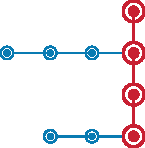
\includegraphics[]{grafikk/toc.pdf}
	
\addtocounter{framenumber}{-1}
\thispagestyle{empty}
\end{frame}










\begin{frame}\label{fr:bymiljoetaten}
	\frametitle{Om Bymiljøetaten}
	\usebeamerfont{text}
	Bymiljøetaten er den delen av Oslo kommune som har ansvar for  \alert{planlegging, utvikling, forvaltning og drift} av kommunale byrom i Oslo. Her inngår alt fra veier og torg til parker og friområder. De har også ansvar for kommunale idrettsanlegg.

	Bymiljøetaten er delt inn i fire divisjoner, miljø-, bydrifts-, kunde- og utviklingsdivisjonen. Ettersom vi jobbet med parkering var det bydriftsdivisjonen vi jobbet opp mot.
	
	\vspace{5em}
	\centerline{\includegraphics[scale=0.5]{grafikk/oslo_kommune.jpg}}
\end{frame}











\begin{frame}\label{fr:begreper}
	\frametitle{Begreper}
	\usebeamerfont{text}
	
	\vspace{1em}
	
	\begin{beamercolorbox}[wd=0.60\textwidth, ht=5.5ex, dp=5pt, leftskip=.3cm, rightskip=.3cm]{begrep1}
		\tiny
		\textbf{Parkering:} Å sette fra seg kjøretøyet sitt. I vår betydning på oppmerkede plasser i byen, enten avgiftsbelagte eller ikke.
	\end{beamercolorbox}
	
	\vspace{-1em}
	
	\hfill\begin{beamercolorbox}[wd=0.70\textwidth, ht=5.5ex, dp=5pt, leftskip=.3cm, rightskip=.3cm]{begrep2}
		\tiny
		\textbf{Parkeringsvakt/kontrollør:} Ansatte hos Bymiljøetaten som har som oppgave å sjekke om bilene står lovlig parkert. Deler ut bøter ved avvik.
	\end{beamercolorbox}
	
	\begin{beamercolorbox}[wd=0.90\textwidth, ht=10ex, dp=5pt, leftskip=.3cm, rightskip=.3cm]{begrep3}
		\tiny
		\textbf{Lovlig parkert bil:}  (1) Hvis plassen er betalingsbelagt skal føreren av kjøretøyet ha betalt parkeringsavgiften. (2) En bil som står innenfor det avgrensa området markert som parkeringsplass. (3) Hvis parkeringsplassen har en tidsbegrensning på P-plassene, så overskrider ikke kjøretøyet denne.
	\end{beamercolorbox}
	
	\vspace{-1em}
	
	\hfill\begin{beamercolorbox}[wd=0.7\textwidth, ht=7.3ex, dp=5pt, leftskip=.3cm, rightskip=.3cm]{begrep4}
		\tiny
		\textbf{Feilparkert bil/parkeringsavvik:} Bil som (1) ikke har betalt parkeringsavgift, (2) ikke står innefor oppmalte linjer, eller (3) har stått for lenge på tidsbegrenset parkering.
	\end{beamercolorbox}
	
	\begin{beamercolorbox}[wd=0.80\textwidth, ht=7.3ex, dp=5pt, leftskip=.3cm, rightskip=.3cm]{begrep5}
		\tiny
		\textbf{System:} System i denne sammenhengen er et komplett parkeringsysstem. Det vil si et sett av komponenter som håndterer og definerer hvordan betaling og kontroll skal foregå, og hvordan avvik skal oppdages. 
	\end{beamercolorbox}
	
	\vspace{-1em}
	
	\hfill\begin{beamercolorbox}[wd=0.80\textwidth, ht=7.3ex, dp=5pt, leftskip=.3cm, rightskip=.3cm]{begrep6}
		\tiny
		\textbf{Interessenter:} Med interessenter mener vi de forskjellige aktørene som på et eller annet vis berøres av et nytt system. Disse er: Bymiljøetaten i Oslo, bilister som kommer til å bruke parkeringsplassene, samt parkeringsvakter.
	\end{beamercolorbox}

\end{frame}








\begin{frame}\label{fr:metodikk}
	\frametitle{En iterativ prosess}
	\usebeamerfont{text}
	Gjennom prosjektet har vi hatt som hovedfokus å \alert{forstå} kundens faktiske \alert{behov}. Da gruppa 
valgte oppgaven, var førsteprioritet å få et så godt \alert{overblikk} som mulig over parkeringssituasjonen i Oslo, og hva intensjonene bak deres påtenkte nye parkeringssystem var. Gjennom e-poster, telefonsamtaler, møter og seminar ble vårt formål i forbindelse med Oslo Bymiljøetats prosjekt gradvis \alert{konkretisert}.

	Fremgangsmåten har vært preget av en \alert{iterativ} prosess. Etter å ha dannet oss inntrykk av kundens ønsker, fremla vi hvordan vi tolket det som kom fram. På denne måten forsikret vi oss om at vi til enhver tid hadde \alert{forankring} i kundens behov. Da vi etterhvert følte at vi hadde forstått deler av behovene, begynte vi å tenke på hvordan vi kunne få \alert{ytterliggere kunnskap} rundt temaet.
	
	I faget Innovasjon har \alert{Doblins ti innovasjonstyper} vært et sentralt tema. Innovasjonsselskapet Doblin utviklet mot slutten av 90-tallet en modell som deler innovasjon inn i ti kategorier. Grovt sett kan disse kategoriseres i hva man leverer, hvilke rammeverk en har for å levere, og hvordan brukeren opplever tjenestene og produktene som leveres.

	\bigskip
	\centerline{\includegraphics[scale=0.9]{grafikk/various/doblin.pdf}}
\end{frame}














\begin{frame}
	\usebeamerfont{text}
	Etter et møte med Bymiljøetaten i Oslo, satt gruppen igjen med inntrykk av at vi hovedsakelig befant oss på kategorien som handlet om hva man leverer, der \alert{produktytelse og produktsystem} inngår. For å undersøke hvorvidt dette inntrykket stemte, samt å konkretisere problemstillingen gruppen skulle jobbe med, skisserte vi i samråd med veileder Chris Klemmetsvold \alert{seks problemstillinger} vi anså som relevante for prosjektet:
	
	\hspace{2em}\alert{1.} \emph{Hvordan kan avvik \alert{oppdages} på en mer effektiv måte enn det gjøres per dags dato?} \\
	\hspace{2em}\alert{2.} Hvordan kan man sikre at en bruker alltid har tilgang til å parkere på sin \alert{beboerparkering} ved behov?  \\
	\hspace{2em}\alert{3.} Hvordan gjøre det enklere for bruker å \alert{betale} for å unngå avvik?  \\
	\hspace{2em}\alert{4.} Hvordan \alert{samordne} betalingsløsningene for å effektivisere kontroll?  \\
	\hspace{2em}\alert{5.} Hvordan \alert{redusere} antallet feilparkeringer?  \\
	\hspace{2em}\alert{6.} Hvordan kan parkeringssystemet gjøres mest mulig \alert{automatisert}?
	
	Etter videre dialog ble det bestemt at gruppen skulle fokusere på \alert{problemstilling 1}, med følgende begrunnelse fra Bymiljøetaten i Oslo, ved John Toverød: 
	
	\hspace{2em}\begin{beamercolorbox}[wd=0.75\paperwidth, ht=8ex, dp=8pt, leftskip=.3cm, rightskip=.3cm]{quotecolor}
	\huge`` \\[-0.5em]
    \tiny
    \hspace{1.5em}\vspace{0.0em}\emph{I dag brukes store ressurser på å kontrollere kjøretøy som står lovlig parkert. Vi ønsker å dreie ressursbruken over på kontroll av avvikene.} \\ [-1.8em]
    
    \hspace{0.70\paperwidth}\huge'' \\ [-0.3em]
\end{beamercolorbox}

Det å \alert{forstå dagens system} sett fra parkeringskontrollørenes perspektiv, ville tilført oss verdifulle opplysninger når vi senere skulle komme frem til mulige løsninger. Å lytte til folk med sterke meninger rundt det man ser på, er viktig i en innovasjonsprosess for å få en kvalitativ forståelse av behovene. Oslo Bymiljøetat ønsket \emph{ikke} at vi skulle kontakte parkeringskontrollører, da prosjektet foreløpig var \alert{forbeholdt styret}. På grunnlag av denne tilbakemeldingen, ble det for gruppen klart at kunden selv ønsket å gjennomføre undersøkelser i forbindelse med prosjektet, og at \alert{vår oppgave var å finne mulige løsninger}.
\end{frame}










\begin{frame}
	\usebeamerfont{text}
	Arbeidsprosessen kan oppsummeres ved hjelp av suksessformelen:
	\vspace{-2em}\begin{center}
		{\footnotesize%
			Suksess \alert{=} behov \alert{$\times$} verdi \alert{$\times$} ildsjel \alert{$\times$} team \alert{$\times$} forankring
		}
	\end{center}\vspace{-2em}
	\alert{Behov:} Vi har hatt fokus på å avdekke kundens behov. Det har vært utfordringer knyttet til dette, spesielt i forhold til at behovet kunden fremstiller ikke nødvendigvis er det samme som den ønsker å oppnå. Vi har hatt begrensede muligheter for å sjekke dette samsvaret. \\ [1em]
	\alert{Verdi:} Verdi er i innovasjonsfaget definert som oppfyllelse av behov, minus heft. Ettersom vi ikke får se løsningen satt ut i live, har vår vurdering av verdi vært preget av gruppens subjektive synsing, basert på informasjon fra Bymiljøetaten. Heft: stor engangsutgift, opplæring i nytt system, vedlikehold, nye utfordringer knyttet til den nye teknologien.  \\ [1em]	
	\alert{Ildsjel:} Det har ikke vært noen åpenbar ildsjel i prosjektet. For gruppens vedkommende, har nok distansen til prosjektet vært hovedårsak. I Bymiljøetaten virker det som om ansvaret muligens er fordelt på for mange personer.  \\ [1em]	
	\alert{Team:} Teamet består av fem sivilingeniørstudenter ved NTNU med spesialisering i fagfeltene kjemi, petroleumsteknologi, geomatikk, produktutvikling og IKT. Ingen hadde tidligere erfaring med parkeringssystemer da prosjektet startet.  \\ [1em]	
	\alert{Forankring:} Vi har til enhver tid inkludert Bymiljøetaten mest mulig. Hovedsakelig har kommunikasjonen foregått med kontaktpersonene John Toverød og Kjetil Storaas Hansen.	
\end{frame}










\begin{frame}\label{fr:kundebehov}
	\frametitle{Kundens behov}
	\usebeamerfont{text}
	Etter flere samtaler med kunden og flere ompriorteringer underveis, har vi kommet frem til at Bymiljøetatens viktigste behov er å \alert{minske mengden ressurser som brukes på parkeringskontroll}. 
	
	Kontrollen i dag tar \alert{lang tid}, og er \alert{lite effektiv}: kontrollørene må sjekke hver eneste bil og manuelt gjøre oppslag i flere \alert{forskjellige databaser}. Veldig mye tid går med på å sjekke \alert{lovlig} parkerte biler. Det er et ønske om et system som \alert{synliggjør avvikene}. Det er samtidig et ønske om å kunne implementere dette \alert{raskt}, ettersom dette skal utprøves i et pilotprosjekt med \alert{beboerparkering}. 
	
		Vi har, ut fra de avdekte behovene satt opp kriterier for et \alert{ideelt system}, og undersøkt hvordan eksisterende systemer for parkeringsovervåkning oppfyller disse. 	Det er lagt spesielt stor vekt på innføring av teknologi i denne undersøkelsen. Dette er et sterkt ønske fra Bymiljøetatens side som kom klart fram under et møte.
	
	\vspace{1.5em} 

	\begin{beamercolorbox}[wd=0.33\paperwidth,ht=14ex,dp=5pt,leftskip=.3cm,rightskip=.3cm]{quotecolor}
	\huge`` \\[-0.5em]
    \tiny
    \hspace{1.5em}\vspace{0.0em}\emph{Vi er klar over at vi i kommunen er fryktelig sirumpa, men nå skal vi virkelig ta av!} \\ [-1.8em]
    
    \hspace{0.27\paperwidth}\huge'' \\ [-0.3em]
    
    \hfill\tiny- Anonym kommunal ansatt \\ [1em] % Kjetil Storås Hansen
\end{beamercolorbox}

		\hfill\begin{beamercolorbox}[wd=1.0\textwidth, ht=10ex, dp=10pt, leftskip=.3cm, rightskip=.3cm]{lesmer}
	\textbf{Beboerparkering} er en løsning hvor beboere i en bydel kan få tilgang til en fleksibel (ikke fast) parkeringsplass i gata mot betaling. Hensikten med beboerparkering er å sikre best mulig tilgjengelighet til offentlige parkeringsplasser for beboere i bydelene.
\end{beamercolorbox}	
\end{frame}








\begin{frame}\label{fr:problemstilling}
	\frametitle{Problemstilling}

	\hspace{20em}{\usebeamerfont{illustrative}\color{MatteYellow}?}\\ [-10.5em]
	Hvordan kan parkeringskontroll \alert{effektiviseres} med teknologi?
	
	\usebeamerfont{text}
	\textbf{Rammer:}
	\begin{itemize}
		\item Løsningen er tenkt implementert innen \alert{kort tid}.
		\item Løsningen skal være \alert{fremtidsrettet}, med gode muligheter for \alert{videreutvikling}.
		\item Løsningen bør ikke kreve mer \alert{ressurser} enn den frigjør.
		\item Løsningen tar ikke hensyn til om kjøretøyet står lovlig parkert i forhold til oppmerking og skilting.
	\end{itemize}
\end{frame}








\begin{frame}\label{fr:dagens_situasjon}
	\frametitle{Dagens situasjon}
	\usebeamerfont{text}
	
		\begin{columns}[onlytextwidth]
		\begin{column}{0.60\textwidth}
			I dag må vaktene bevege seg rundt og \alert{kontrollere alle biler}, uavhengig av  om de er feilparkert eller ikke. De kan sjekke om det finnes en papirbillett i vinduet. Dersom dette ikke finnes må de bruke en håndholdt enhet for å sjekke om parkeringen er betalt elektronisk. De må også gjøre \alert{manuelt oppslag i flere databaser}, en etter en, for å sjekke om piggdekksavgift er betalt, miljøagvift, etc. Parkeringsvaktene føler at dette er veldig \alert{lite effektivt}. \\ [1em]
	
	For bilistene er det i dag ofte svært \alert{vanskelig å finne en ledig parkeringsplass}. Dette fører til at folk ofte kjører lenge rundt for å finne et sted å parkere, noe som fører til mer \alert{forurensning}. Det gjør også at bilister i større grad er villige til å bevisst parkere ulovlig. Mange er også usikre på om de parkerer lovlig, mye grunnet mangelfull oppmerkning. Dette fører til en del \alert{unødvendige parkeringsavvik}.
		\end{column}
		\begin{column}{0.35\textwidth}
	\hspace{16em}\begin{beamercolorbox}[wd=0.33\paperwidth,ht=17ex,dp=3pt,leftskip=.3cm,rightskip=.3cm]{quotecolor}
	\huge`` \\[-0.5em]
    \tiny
    \hspace{1.5em}\vspace{0.0em}\emph{Noen ganger er det så vanskelig å finne parkeringsplass at jeg parkerer feil med vilje.} \\ [-1.8em]
    
    \hspace{0.27\paperwidth}\huge'' \\ [-0.3em]
    
    \hfill\tiny- Chris Klemmetvold \\ [1em] % Kjetil Storås Hansen
\end{beamercolorbox}
	
			\vspace{2em}\includegraphics[angle=30]{grafikk/feilparkering.pdf}
		\end{column}
	\end{columns}
	
\end{frame}









\begin{frame}\label{fr:kundereise}
	\frametitle{Hvor skoen trykker}
	\usebeamerfont{text}
	Det er \alert{essensielt at løsninger tilpasses et reelt behov}, og da må man vite hvor skoen trykker. 
	
	En kundereise er et hjelpemiddel som brukes for å kunne danne et \alert{helhetlig} bilde av hvilke stadier kunder går gjennom ved bruk av tjenester. Det er et mye brukt verktøy i tjenestedesign for å forstå \alert{kunders behov}, og å gi innsikt om hvordan en løsning best mulig kan oppfylle disse for å skape \alert{verdi} hos kunden. Her ser man ikke på små tekniske detaljer, men de viktigste stadiene kunden må gjennom både før, under og etter at han benytter seg av tjenesten. 

	En kundereise kan hjelpe med å løfte blikket fra enkeltproduktene, og heller se på hvordan kunden opplever de forskjellige stadiene i tjenesten som tilbys. Slik kan det også åpne for samarbeid mellom forskjellige avdelinger i organisasjonen. 

	Merk at kundereisene vi viser her er mangelfulle. En kundereise fungerer best mulig når det er innhentet tilfredsstillende mengder informasjon. Mer informasjon ville også gjort det mulig å bedre karakterisere de forskjellige gruppene som omfattes av begrepet “bilist”, da det er forskjellige behov blandt pendlere, turister, beboere, bedrifter og andre undergrupper. 



	\hfill\begin{beamercolorbox}[wd=0.69\textwidth, ht=6.8ex, dp=10pt, leftskip=.3cm, rightskip=.3cm]{lesmer}
	Hvis du vil lese mer om kundereise som et verktøy, finner du det her:
	\emph{http://blog.makingwaves.no/ideer/hvordan-ser-kundereisen-ut/}
\end{beamercolorbox}
\end{frame}









\begin{frame}\label{fr:bilisters_hverdag}
	\bigskip
	\centerline{{\large Bilisters hverdag}}
	\vspace{1.5em}
	\centerline{\includegraphics[]{grafikk/kundereiser/bilist_foer.pdf}}
\end{frame}










\begin{frame}\label{fr:kontrollorers_hverdag}
	\centerline{{\large Kontrollørers hverdag}}
	\vspace{2.5em}
	\centerline{\includegraphics[]{grafikk/kundereiser/kontrolloer_foer.pdf}}
\end{frame}





\begin{frame}\label{fr:ideelt_system}
	\section{Et ideelt system}
	\frametitle{Et ideelt system}
	\usebeamerfont{text}
	Et ideelt system skal \alert{oppfylle så mange av Bymiljøetatens krav som mulig}. Systemet bør ikke være for kostbart å innføre, og inkludert vedlikeholdsarbeid bør det nye systemet være \alert{arbeidsbesparende}.
	
	\begin{itemize}
	\item Systemet gjør det \alert{enklere for bilister} å parkere forskriftsmessig. Dette vil gi mer fornøyde sluttbrukere, og samtidig redusere arbeidsmengden for parkeringsvaktene.
	\item Systemet \alert{reduserer parkeringsvaktenes arbeid} med å kontrollere fullgode parkeringer gjennom automatisering. Dette vil gjøre arbeidsdagen deres enklere og mer effektiv.
	\item Systemet er totalt sett, over tid, \alert{besparende} for Bymiljøetaten i Oslo.
	\end{itemize}

	Gruppen anser det som hensiktsmessig for Bymiljøetaten å analysere parkeringskontrollørene og bilistene sine behov og forventninger til et nytt system, da det er disse gruppene som vil bli mest direkte rammet. Det nye systemets suksess avhenger av at disse gruppene føler at deres behov ivaretatt. Vi oppfordrer Bymiljøetaten til å gjøre alle vurderinger i lys av dette, og ikke ene og alene ha fokus på hva som er den beste teknologien.
	
	\vspace{3em}
	\hspace{20em}\includegraphics[scale=0.6]{grafikk/dummy/circ1.pdf}\\ [-2em] 
	\hspace{25em}\includegraphics[scale=0.3]{grafikk/dummy/circ2.pdf}\\ [-5em]
	\hspace{30em}\includegraphics[scale=0.5]{grafikk/dummy/circ3.pdf}\\ [-6em]
	\hspace{35em}\includegraphics[scale=0.7]{grafikk/dummy/circ4.pdf}\\ [-3em]
	\hspace{40em}\includegraphics[scale=0.4]{grafikk/dummy/circ5.pdf}
\end{frame}



\begin{frame}\label{fr:eksiterende_losninger}
	\section{Eksisterende teknologiske løsninger}
	\frametitle{Eksisterende teknologiske løsninger}
	\usebeamerfont{text}
	Vi har sett på tre eksisterende systemer som i stor grad oppfyller behovet om automatisk varsling av avvik. De tre systemene er ganske like, men hver av de har sine fordeler. Merk at informasjonen som er oppgitt her stort sett er begrenset til informasjonen på nettsidene til produsentene, ettersom vi kun har fått kontakt med Smart Parking.
	\vspace{2em}
	
	\begin{columns}[T]
		\begin{column}{0.33\textwidth}
			{\footnotesize\alert{Fybr}}
			\begin{itemize}
				\item Amerikansk leverandør.
				\item Brukes i San Francisco.
				\item Sensor med \alert{radar og magnetometer}.
				\item Systemet består av sensorer og reléer, samt \alert{apper for bilister og kontrollører} og webbasert administrasjonssystem.
			\end{itemize}
		\end{column}
		\begin{column}{0.33\textwidth}
			{\footnotesize\alert{Smart Parking}}
			\begin{itemize}
				\item Global leverandør med kontor i Storbritannia.
				\item Brukes i bl.a. Westminster, Manchester (UK) og Sydney.
				\item Infrarød sensor med \alert{RFID-leser}.
				\item Systemet består av sensorer og reléer, samt app for bilister og administrasjonssystem.
			\end{itemize}
		\end{column}
		\begin{column}{0.33\textwidth}
			{\footnotesize\alert{Urbiotica}}
			\begin{itemize}
				\item Spansk leverandør.
				\item Brukes i Nice.
				\item Sensor med magnetometer og lysmåler.
				\item Systemet består av sensorer, to lag med reléer og administrasjonssystem.
				\item Mulighet for utvidelser.
			\end{itemize}
		\end{column}
	\end{columns}
	
		\hfill\begin{beamercolorbox}[wd=0.35\textwidth, ht=5ex, dp=5pt, leftskip=.3cm, rightskip=.3cm]{defcolor}
    \tiny
    \textbf{Relé}: En enhet som har ansvar for videresending av informasjon.
	\end{beamercolorbox}\hfill
	\begin{beamercolorbox}[wd=0.60\textwidth, ht=10ex, dp=5pt, leftskip=.3cm, rightskip=.3cm]{defcolor}
    \tiny
    \textbf{RFID}: Radiofrekvensidentifikasjon. En metode for å lagre og hente data i små brikker. Brikkene inneholder antenner slik at de kan motta og svare på radiofrekvenssignaler fra en RFID sender.
	\end{beamercolorbox}
\end{frame}




\begin{frame}\label{fr:fybr}
	\subsection{Fybr}
	\frametitle{\alert{Fybr}}
	\usebeamerfont{text}
	\emph{Fybr} er en amerikansk leverandør av parkeringssystemer med nærmere 15 års erfaring med \alert{sensorbaserte parkeringssytemer}. Systemet deres er i bruk i San Francisco.
	
	Parkeringssystemet de leverer består av \alert{sensorer} som plasseres i bakken. Sensorene kommuniserer trådløst med \alert{reléer} som monteres på lyktestolper. Dette er knyttet opp mot et datasystem som tilbyr \alert{analyseverktøy} for Bymiljøetaten og \alert{mobilapper} for kontrollører og brukere. 
	
	Systemet registrerer overganger, altså når en bil ankommer og forlater en parkeringsplass. Det har oversikt over hvor lenge en bil har stått på en parkeringsplass, som er svært nyttig for områder med \alert{tidsbegrenset parkering}. Fybr leverer også egenutviklede \alert{parkometre} som registrerer betaling i systemet.
	
	Sensorene benytter både \alert{magnetometer og radar} for å registre biler. De er batteridrevne, og kommuniserer med reléer montert høyt oppe på stolper. Batterilevetiden for sensorene er opp til \alert{fem år}.
	
	\vfill\hfill\includegraphics[scale=0.3]{grafikk/logoer/fybr.png}
\end{frame}


\begin{frame}	
	\hfill\includegraphics[scale=0.3]{grafikk/logoer/fybr.png} \\ [-10em]
	\begin{center}{\large Fybrs programvarepakke}\end{center}
	\usebeamerfont{text}
	\begin{columns}[onlytextwidth]
		\begin{column}{0.5\textwidth}
			Datasystemet som følger med Fybrs parkeringssystem består av tre verktøy:
	
			\begin{itemize}
				\item \emph{Parking Genius}, en mobilapp for iPhone og Android  som \alert{gir bilister oppdatert informasjon} om ledige parkeringsplasser, og viser veien dit.
				\item \emph{Fybr Insights}, et \alert{webbasert administreringssystem} som gir sanntidsinformasjon fra hele systemet, og lar Bymiljøetaten justere priser i sanntid dersom dette er ønskelig.
				\item \emph{Fybr Enforce}, en mobilapp for parkeringsvakter som \alert{varsler når avvik oppstår} og leder dem til det.
			\end{itemize}
		\end{column}
		\begin{column}{0.4\textwidth}
			\emph{Fybr Insights'} muligheter for \alert{prisjustering} er ment å øke sannsynligheten for at det alltid er en ledig plass i et område. Dette gjøres ved at prisene justeres opp i områder med mange opptatte plasser, og ned i områder med mange ledige plasser, noe som oppfordrer folk til å parkere i områder med mindre press.

		\end{column}
	\end{columns}
\end{frame}








\begin{frame}
	\bigskip
	\hfill\includegraphics[scale=0.3]{grafikk/logoer/fybr.png} \\ [-1em]
	\bigskip
	\centerline{\includegraphics{grafikk/eksisterende_systemer/fybr_smaller.pdf}}
\end{frame}








\begin{frame}\label{fr:smart_parking}
	\subsection{Smart Parking}
	\frametitle{\alert{Smart Parking}}
	\usebeamerfont{text}
	\emph{Smart Parking} er en global leverandør av parkeringsløsninger, og har et av sine \alert{kontorer i Storbritannia}. De har tidligere deltatt i flere byparkeringsprosjekter i blant annet \alert{Westminster}, \alert{Manchester} (UK) og \alert{Sydney}.
	
	Systemet består av \alert{sensorer} som plasseres i bakken. Sensorene kommuniserer trådløst med stolpemonterte \alert{reléer}. Disse reléene sender informasjonen videre til et sentralt datasystem gjennom \alert{3G} nettet. Datasystemet videreformidler denne informasjonen til bilister gjennom en \alert{app}, og til Bymiljøetatens \alert{overvåkningsprogramvare}.
	
	Smart Parking sine sensorer, kalt \emph{SmartEye}, bruker \alert{infrarød} teknologi for å oppdage om parkeringsplassen er okkupert. Sensorene kan også leveres med \alert{RFID leser}, som sammen med en brikke plassert i bilen kan brukes til å automatisere betaling. Sensorene har en batterilevetid på omtrent \alert{fem år}. I tillegg til dette leverer Smart Parking egenutviklende \alert{parkometre} som registrerer betalingen i systemet.
	\vfill\hfill\includegraphics[scale=0.2]{grafikk/logoer/smartparking.png}
\end{frame}








\begin{frame}
	\bigskip
	\vfill\hfill\includegraphics[scale=0.2]{grafikk/logoer/smartparking.png} \\ [-1em]
	\centerline{\includegraphics{grafikk/eksisterende_systemer/smartpark_smaller.pdf}}
\end{frame}








\begin{frame}\label{fr:urbiotica}
	\subsection{Urbiotica}
	\frametitle{\alert{Urbiotica}}
	\usebeamerfont{text}
	Urbiotica er en \alert{spansk} leverandør av sensorer for bruk i byinfrastruktur. De har hatt et stort parkeringsprosjekt i \alert{Nice}, der over \alert{ti tusen} parkeringsplasser er overvåket med sensorer.
	
	Systemet de leverer består av sensorer, kalt \alert{\emph{U-Spot}}, som plasseres i bakken. Sensorene kommuniserer trådløst med \alert{\emph{U-flag}}, en liten boks som monteres på nærliggende lyktestolper. Den trådløse rekkevidden mellom sensorene og U-flag er på inntil 50 meter. U-flag kommuniserer videre, med en rekkevidde på inntil 100 meter, til en annen lyktestolpemontert boks, kalt \alert{\emph{U-box}}. U-box videreformidler til slutt dataene til Urbioticas programvareplatform, \alert{\emph{U-base}}, via WiFi.
	
	
	Sensorene bruker \alert{magnetometer og lyssensor} for å registrere om det står en bil parkert på plassen. Sensorene tåler ned til \alert{-20$\textdegree$C}. Batterilevetiden er oppgitt å være opp til \alert{ti år}. Installasjonen av hver enkelt sensor kan gjøres på i underkant av \alert{ti minutter}.

	Programvaren som leveres med systemet kalles \alert{\emph{U-Admin}}. Dette gir Bymiljøetaten en \alert{visuell fremstilling} av de innsamlede dataene og \alert{varsler ved eventuelle feil} i systemet. Systemet har også mulighet for \alert{deling av data} med andre applikasjoner, som for eksempel \alert{mobilapper}. 
	
		Ettersom Urbioticas system er laget for å kunne overvåke mer enn bare parkering, er det gode muligheter for \alert{utvidelser}. Man kan bl.a. overvåke nivået i søppelkontainere, luftfuktighet og generell trafikkflyt i byen.
	
	\vfill\hfill\includegraphics[scale=0.2]{grafikk/logoer/urbiotica.jpg}
\end{frame}









\begin{frame}
	\bigskip
	\vfill\hfill\includegraphics[scale=0.2]{grafikk/logoer/urbiotica.jpg} \\ [-1em]
	\bigskip
	\centerline{\includegraphics{grafikk/eksisterende_systemer/urbiotica_smaller.pdf}}
\end{frame}









\begin{frame}\label{fr:kvalitativ_sammenligning}
	\frametitle{Kvalitativ sammenligning av systemene}
	\usebeamerfont{text}
	Neste side viser en grafisk fremstilling av Fybr, Smart Park og Urbioticas egenskaper, og hvordan ulike interessenter verdsetter dem. Hver faktor vurderes på en skala fra 1 til 10, der 10 er best. De vurderte faktorene er som føgler:
	
	\begin{tabular}{lp{8.5cm}}
	\alert{Erfaring} 			& Tidligere relevante erfaringer med implementasjon av deres respektive system.  \\ [1em]
	\alert{Norsk klima} 		& Hvor godt utstyret til leverandørene takler norske værforhold. Tar i betraktning hvor godt utstyret vil fungere om vinteren, samt om det rent teknisk vil overleve kulden.
 \\ [1em]
	\alert{Kompleksitet} 		& Systemets kompleksitet. Høyere verdi tilsvarer et mindre komplekst system. Skalaen er snudd fordi et system som består av mange komplekse ledd vil være vanskeligere å vedlikeholde og reparere.
 \\ [1em]
	\alert{Fleksibilitet} 		&Hvor fleksibel løsningen er i forhold til videreutvikling i form av applikasjoner for brukere/kontrollører, og hvor gode muligheter det er for å tilpasse systemet etter Bymiljøetatens behov.
 \\ [1em]
	\alert{Verdi for brukere} 	& Hva systemet tilbyr brukerene, altså bilistene. Et av momentene  som gir høyere verdi, er applikasjon for å hjelpe brukere med å finne en ledig parkeringsplass.
 \\ [1em]
	\alert{Verdi for vakter} 	& Hvor gode hjelpemidler systemet har i forhold til å gjøre kontrollørenes jobb lettere. Hvis det f.eks. finnes smarte løsninger integrert i systemet for å varsle om avvik vil dette gi et positivt utslag.
 \\
	\end{tabular}
\end{frame}









\begin{frame}
	\centerline{\includegraphics{grafikk/grafer/analyse.pdf}}
\end{frame}









\begin{frame}\label{fr:begrunnelse}
	\begin{center}
		\large{Begrunnelse}
	\end{center}
	\usebeamerfont{text}
	
	\begin{tabular}{llp{7cm}}
	\alert{Fybr} 			& \emph{Erfaring} 		& Fybrs system er i bruk i \alert{San Fransisco}. \\ [0.5em]
							& \emph{Norsk klima}	& Fybrs sensorer med radar og magnetometer \alert{bør fungere godt gjennom snø og is}, men de oppgir ikke om systemet tåler kulde. \\
							& \emph{Fleksibilitet}	& Fybrs system ser ikke ut til å være veldig fleksibelt, men det ser ut til at systemet med små modifikasjoner kan utvides til å lese RFID brikker. \\
							& \emph{Verdi for brukere} & App viser bilister vei til ledige parkeringsplasser. \\ [0.5em]
							& \emph{Verdi for vakter} & Egen \alert{app for parkeringsvakter} varsler om parkeringsavvik. \\ [2em]
	\alert{Smart Parking} 	& \emph{Erfaring} 		& Smart Parking sitt system er hittil implementert i små byer og på kjøpesentre, flyplasser etc. De har i tillegg nylig inngått en avtale om å implementere systemet for 10 000 parkeringsplasser i Westminster. \\ [0.5em]
							& \emph{Norsk klima} 	& Smart Parking sine sensorer \alert{fungerer \emph{ikke} gjennom snø og is}. Systemet \alert{tåler \emph{ikke} temperaturer under 0$\textdegree$C}.  \\ [0.5em]
							& \emph{Fleksibilitet} 	& Mulighet for å bruke \alert{RFID brikker} til automatisk betaling trekker opp. \\ [0.5em]
							& \emph{Verdi for brukere} & RFID brikke i bilen sørger for \alert{automatisk betaling}. \\ [0.5em]
							& \emph{Verdi for vakter} & Håndholdt terminal for vaktene som brukes til kontroll. \alert{Trolig vanskelig å integrere med eskisterende databaser}. \\ [0.5em]
	\end{tabular}
\end{frame}









\begin{frame}
	\vspace{4em}
	\usebeamerfont{text}
	\begin{tabular}{llp{7cm}}
		\alert{Urbiotica} 	& \emph{Erfaring} 		& Urbioticas system \alert{brukes på 10 000 parkeringsplasser i Nice}, samt flere andre steder. \\ [0.5em]
							& \emph{Norsk klima} 	& Magnetometeret i Urbioticas sensorer \alert{bør fungere gjennom snø og is}. Det er oppgitt at systemet \alert{fungerer ned til -20$\textdegree$C.} \\ [0.5em]
							& \emph{Fleksibilitet} 	& Urbioticas system er \alert{fleksibelt} mtp. å legge til overvåkning av f.eks. kontainere og generell trafikkflyt. \\ [0.5em]
							& \emph{Verdi for brukere} & Åpen API gjør det mulig å lage apper o.l. \\ [0.5em]
							& \emph{Verdi for vakter} & Åpen API gjør at man kan lage et eget, tilpasset system. \\
	\end{tabular}
	
	\vspace{4em}
	\hspace{20em}\includegraphics[scale=0.5]{grafikk/dummy/circ5.pdf}\\ [-3.5em] 
	\hspace{25em}\includegraphics[scale=0.5]{grafikk/dummy/circ4.pdf}\\ [-3.5em]
	\hspace{30em}\includegraphics[scale=0.5]{grafikk/dummy/circ3.pdf}\\ 
	\vspace{5em}
	
	\vspace{3em}
	\hfill\begin{beamercolorbox}[wd=0.50\paperwidth, ht=5.5ex, dp=5pt, leftskip=.3cm, rightskip=.3cm]{defcolor}
    \tiny
    \textbf{API}: Fra Application Programming Interface. “Kanal” som gir mulighet for å hente rådata ut av systemet.

	\end{beamercolorbox}	
\end{frame}










\begin{frame}\label{fr:analyse_av_losningene}
	\frametitle{Analyse av løsningene}
	\usebeamerfont{text}
	\alert{Smart Parking} er, slik systemet fremstår i dag, \alert{uaktuelt}. Dette fordi sensorene ikke fungerer gjennom snø/is, og kommunikasjonsenhetene tåler ikke vinterkulden. Hvis vi ser bort fra dette, er Smart Parking sitt system det som passer Bymiljøetatens ønsker best, ettersom dette er det eneste med støtte for identifiseringsbrikker i bilen.
	
	\alert{Urbiotica} er godt utprøvd, og systemet fungerer ned til minimum -20$\textdegree$C. Et problematisk punkt er at de magnetiske sensorene kan gi feil målinger dersom sensoren er plassert i nærheten av elektrisk utstyr. Lyssensoren kan ikke korrigere for dette på vinteren. Systemet har ingen tilhørende programvare for bilister og kontrollører i felten, men det er lagt opp til at det lett kan utvikles programvare som nyttegjør data fra systemet. Systemet er i dag et rent sensorsystem uten noen betalingsløsning, men systemet er rimelig fleksibelt, derfor er tilpasninger som dette trolig uproblematiske.
	
	\alert{Fybr} sine sensorer bør, rent teknisk, fungere svært bra gjennom is og snø. Men Fybr oppgir ikke noen informasjon om hvilket temperaturområde systemet fungerer i. Systemet ser heller ikke ut til å ha blitt brukt/testet i noe klima som kan sammenlignes med det norske. Systemet inkluderer apper som gjør det lettere for bilister å finne ledige plasser og for kontrollører å oppdage avvik. Det har i tillegg mulighet for prisjustering i sanntid, noe som øker sannsynligheten for at det finnes en ledig parkeringsplass i hver sone: bilister "oppmuntres" til å parkere i soner med lite press. Dette gjør igjen at folk ikke trenger å kjøre så mye rundt for å finne parkeringsplass. Systemet ser ut til å være heller lite fleksibelt mtp. betalingsløsning: man kan betale med app, eller med Fybrs egenutviklede parkometere.
\end{frame}










\begin{frame}\label{fr:anbefalning}
	\frametitle{Anbefaling}
	%\hspace{20em}{\usebeamerfont{illustrative}\color{MatteYellow}!}\\ [-10.5em]
	\usebeamerfont{text}
	Vi har vurdert de tre systemene Smart Parking, Urbiotica og Fybr. Alle de tre systemene har mangler eller begrensninger, men \alert{Fybrs} system skiller seg ut som det som krever færrest endringer.
	
	Fybrs \emph{sensorer} er de \alert{beste for norske forhold} av de tre vi har sett på, men Fybr oppgir ikke om systemet fungerer ved lave temperaturer. Sensorene mangler støtte for lesing av identifiseringsbrikker, men med tanke på at dette er et stort prosjekt anser vi det som sannsynlig at Fybr er villige til å legge til støtte for dette.
	
	\vspace{2em}
	
	\hfill\includegraphics[scale=1.0]{grafikk/recomended.pdf}
\end{frame}










\begin{frame}\label{fr:alternative_losninger}
	\section{Alternative løsninger}
	\frametitle{Alternative løsninger}
	\usebeamerfont{text}
	
	Det å implementere et omfattende parkeringskontrollsystem er en \alert{dyr og tidkrevende} prosess. Derfor har vi valgt å nevne noen relativt enkle tiltak som kan bedre dagens situasjon uten store omkostninger.
	
	{\footnotesize\alert{Oppdatere programvaren på de håndholdte enhetene}}\\
	Et grep Bymiljøetaten kan gjøre er å \alert{oppdatere programvaren til de håndholdte enhetene} kontrollørene bruker daglig. Dersom programvaren oppdateres til å \alert{automatisk} gjøre oppslag for alle relevante databaser samtidig, i stedet for at det gjøres manuelt, vil det korte ned tiden kontrollørene bruker på hver bil.
	
	{\footnotesize\alert{Sivilkontrollører}}\\
	Alle de foreslåtte systemene vi har tatt for oss kontrollerer lovlige parkeringsplasser. Vi er klar over at for å unngå å bli plukket opp som et avvik, kan en parkere et sted hvor det ikke finnes noen sensor og slik unngå å bli kontrollert av systemet. En mulig måte å angripe dette problemet på ville vært å innføre en applikasjon som muliggjør for forbipasserende personer å kunne melde i fra om de værste syndebukkene. 

	Slik det er gjort i \alert{Tyskland}, tror vi kan være til inspirasjon. Her var formålet at syklister og fotgjengere som irriterte seg over at gang- og sykkelstiene ofte var blokkerte av feilparkerte biler skulle kunne melde i fra til kontrollører. 

	Det er ikke nødt til å bli realisert i form av en applikasjon. Hovedtanken bak ideen er at det skal være \alert{lett å gi beskjed om åpenbart feilparkerte biler} og få en kontrollør over for å ordne opp i det. 
\end{frame}










\begin{frame}\label{fr:evaluering}
	\frametitle{Evaluering}
	\usebeamerfont{text}
	{\footnotesize\alert{En ny verden}}\\
	Som det blir beskrevet i innovasjonsfaget, er vi sivilingeniørstudenter vant til å få en 
konkret oppgave og å gå rett til verks med løsningen. I dette prosjektet har vi derimot 
vært avhengig av å snu opp ned på hverdagen slik vi kjenner den. 

		\hspace{11em}\begin{beamercolorbox}[wd=0.50\paperwidth, ht=12ex, dp=6pt, leftskip=.3cm, rightskip=.3cm]{quotecolor}
		\huge`` \\[-0.5em]
		\tiny
		\hspace{1.5em}\vspace{0.0em}\emph{Jeg ville brukt 59 minutter på å definere problemet, 1 minutt på å løse det.} \\ [-1.8em]
		
		\hspace{0.43\paperwidth}\huge'' \\ [-0.4em]
		
		\hfill\tiny- Albert Einstein, om å redde verden på en time \\ [1em] 
	\end{beamercolorbox}

	{\footnotesize\alert{Å avdekke de virkelige behovene}}\\
Det å avdekke kundens behov viste seg å være en større utfordring enn vi hadde 
sett for oss. Utgangspunktet for prosjektet var svært \alert{bredt} og uten klare rammer, noe 
som var en uvant, men samtidig lærerik situasjon for gruppemedlemmene. 

Da vi begynte arbeidet med å avdekke behov, samt å innsnevre problemstillingen, ble vi oppmerksomme på at det var nødvendig å klarere hvem vi skulle ta direkte \alert{hensyn} til, og ikke. Dette endte med å være forbeholdt avdelinger i Bymiljøetaten ettersom prosjektet inngår i en \alert{evaluering på ledelsenivå} i organisasjonen. 

		\vspace{1em}
		
		\hspace{11em}\begin{beamercolorbox}[wd=0.50\paperwidth, ht=12ex, dp=6pt, leftskip=.3cm, rightskip=.3cm]{quotecolor}
		\huge`` \\[-0.5em]
		\tiny
		\hspace{1.5em}\vspace{0.0em}\emph{You've got to start with the customer experience and work back toward the technology - not the other way around.} \\ [-1.8em]
		
		\hspace{0.43\paperwidth}\huge'' \\ [-0.3em]
		
		\hfill\tiny- Steve Jobs \\ [1em] 
	\end{beamercolorbox}
\end{frame}








\begin{frame}
	\usebeamerfont{text}
	Slik vi ser det har Bymiljøetaten vært innstilt på å gjøre \alert{behovsanalysene} knyttet til \alert{interessentene} selv. Bidraget som har vært ønsket fra gruppen har derfor dreid seg om å finne gode forslag til teknologiske løsninger, som Bymiljøetaten selv skal evaluere opp mot behov. Prosjektgruppen for beboerparkering vil ha kartlagt behovene \alert{innen januar 2014}, og derfor ville det vært mer innovasjonsfaglig relevant om gruppens prosjekt hadde startet senere, slik at løsningene var basert på behov også fra interessenter. 

	\alert{Kommunikasjonen} har for det meste foregått via e-post med ulike kontaktpersoner og 
flere divisjoner i Bymiljøetaten. Selv om vi har avlagt to dagsbesøk til Oslo, hadde det vært nyttig med flere telefonsamtaler fremfor e-post. Det kunne også vært fordelaktig med ytterligere \alert{tydelighet} i forhold til hvem vi skulle forholde oss til, da vi hadde inntrykk av at informasjonen tidvis gikk litt på kryss og tvers i Bymiljøetaten.

	\vspace{1.5em}
	\hspace{11em}\begin{beamercolorbox}[wd=0.50\paperwidth, ht=10ex, dp=6pt, leftskip=.3cm, rightskip=.3cm]{quotecolor}
		\huge`` \\[-0.5em]
		\tiny
		\hspace{1.5em}\vspace{0.0em}\emph{Enhver ting kan alltid gjøres bedre enn den blir gjort.} \\ [-1.8em]
		
		\hspace{0.43\paperwidth}\huge'' \\ [-0.3em]
		
		\hfill\tiny- Henry Ford \\ [1em]
	\end{beamercolorbox}
	
	\vspace{1.5em}
	
	Vi ville som tidligere nevnt gjerne hatt mulighet til å gjøre en \alert{grundigere behovsanalyse}, som involverte flere berørte parter. Dette ville gitt et bedre grunnlag for å komme opp med tilpassede løsninger og å vurdere disse opp mot hverandre. Det ville også gitt et større \alert{perspektiv} i forhold til hvilke systemer og funksjoner løsningen burde være, eller kunne gjøres, kompatibel med. 
\end{frame}








\begin{frame}
	\usebeamerfont{text}
	Gjennom prosessen har vi også vært innom mange ulike forslag som ikke har passet 
inn under den endelige problemstillingen og rammene rundt. Dette består gjerne av 
løsninger som vil dekke deler av behovet, og som gruppen anser som relativt \alert{små 
endringer} i forhold til dagens system, med \alert{potensielt stort utbytte}. Et eksempel er å 
samkjøre databasene en kontrollør må sjekke for hver bil (betalingstype, piggdekkavgift 
m.m), og å utvikle kontrollverktøyet til kontrollørene slik at de kun trenger å \alert{scanne skiltet} fremfor å skrive inn skiltnummeret. Dette mener gruppen er en endring som er, relativt 
til innføring av sensorer, lett å implementere og som vil kunne effektivisere kontrollen. 
Ettersom denne løsningen ikke fokuserer direkte på oppdagelse av avvik ble den ikke 
tatt med videre i prosessen.

	En grundigere analyse hadde også vært ønskelig på det økonomiske aspektet. Dette 
har vært vanskelig på grunn av mangel på informasjon rundt det økonomiske både fra 
kunden og fra de tre systemleverandørene. Dette har ikke latt seg gjøre, ettersom vi 
ikke har hatt innsyn i Bymiljøetatens økonomi rundt prosjektet. Hvorvidt Bymiljøetaten 
er interessert i å \alert{redusere antall avvik, og ikke bare oppdage dem mer effektivt}, har vi 
ikke fått kjennskap til. Vi vet ikke om Bymiljøetaten er økonomisk avhengig av bøter 
i budsjettene sine, bare at "alt inngår i en pott". Hvis målet er å også redusere avvik, 
anbefaler vi Bymiljøetaten å også se på tiltak som virker forebyggende, for eksempel 
gjennom å finne ut hvorfor folk parkerer feil. Slik gruppen forstår det, har det ikke vært relevant for Bymiljøetaten å gi oss informasjon rundt økonomi. 
\end{frame}









\begin{frame}
	\usebeamerfont{text}
	{\footnotesize\alert{Videre arbeid}}\\
	I denne prosjektoppgaven er det fokusert på feilparkering grunnet mangelfull betaling. En 
feilparkert bil er også definert ut fra oppmerking og skilting gjennom Vegtrafikkloven, og 
er et interessant område med flere utfordringer som kan undersøkes. Så mye som 75\% 
av alle parkeringsavvik kommer som følge av brudd på Vegtrafikkloven.
En idè kan eksempelvis være å plassere sensorer på områder der ulovlig parkering er et vanlig problem med konsekvenser for annen trafikk.

	"\alert{Hvorfor feilparkerer bilister i Oslo?}" kunne vært en interessant problemstilling for videre 
arbeid rundt Bymiljøetatens nye parkeringssystem.

	{\footnotesize\alert{Suksess?}}\\
	Til syvende og sist er vi fornøyde med de løsningene som har blitt presentert, da 
gruppen anser dette som de mest aktuelle i forhold til behov, problemstilling og rammene 
rundt. Vi er overbevist om at en innføring av sensorteknologi i parkeringskontrollen vil 
gjøre det lettere å oppdage avvik ved feilparkering på grunnlag av betaling og dermed 
gjøre denne prosessen mer effektiv.

	Kanskje hadde gruppens bidrag passet bedre i emnet \emph{\alert{IMAG001 - Konsulenter I Team}}?

\end{frame}









\begin{frame}\label{fr:referanser}
	\frametitle{Referanser}	
	\begin{beamercolorbox}[wd=1.0\textwidth, ht=2.8ex, dp=5pt, leftskip=.3cm, rightskip=.3cm]{refcolor}
    \tiny
    {\usebeamerfont{refhead}\textbf{Beboerparkering:}}\\
	 {\usebeamerfont{reflinkfont}http://www.bymiljoetaten.oslo.kommune.no/trafikk\_og\_samferdsel/parkering/beboerparkering/ \hfill 05.12.2012}
	\end{beamercolorbox}
	
	\begin{beamercolorbox}[wd=1.0\textwidth, ht=2.8ex, dp=5pt, leftskip=.3cm, rightskip=.3cm]{refcolor}
    \tiny
    {\usebeamerfont{refhead}\textbf{Alternative løsninger:}}\\
	 {\usebeamerfont{reflinkfont}http://www.automotorsport.no/2013/10/15/ny-app-gjor-deg-til-parkeringsvakt/ \hfill 15.10.2012}
	\end{beamercolorbox}
	
	\begin{beamercolorbox}[wd=1.0\textwidth, ht=2.8ex, dp=5pt, leftskip=.3cm, rightskip=.3cm]{refcolor}
    \tiny
    {\usebeamerfont{refhead}\textbf{Kundereisen:}}\\
	 {\usebeamerfont{reflinkfont}http://blog.makingwaves.no/ideer/hvordan-ser-kundereisen-ut/ \hfill 30.11.2012}
	\end{beamercolorbox}
	
	\begin{beamercolorbox}[wd=1.0\textwidth, ht=3.6ex, dp=5pt, leftskip=.3cm, rightskip=.3cm]{refcolor}
    \tiny
    {\usebeamerfont{refhead}\textbf{Urbiotica:}}\\
	 {\usebeamerfont{reflinkfont}http://www.urbiotica.com/ \hfill 16.11.2013\\
	 http://www.urbiotica.com/experience/movsmart/  \hfill 17.11.2013}
	\end{beamercolorbox}
	
	\begin{beamercolorbox}[wd=1.0\textwidth, ht=5ex, dp=10pt, leftskip=.3cm, rightskip=.3cm]{refcolor}
    \tiny
    {\usebeamerfont{refhead}\textbf{Smart Parking:}}\\
	{\usebeamerfont{reflinkfont}http://www.smartparking.com/ \hfill 17.11.2013 \\
	http://www.smartparking.com/case-studies/manchester.html \hfill 19.11.2013 \\
	http://www.smartparking.com/case-studies/optus.html \hfill  19.11.2013 \\
	http://www.parking-net.com/parking-news/smart-parking-ltd/westminster-city-council \hfill 26.11.2013 \\}
	\end{beamercolorbox}
	
		\begin{beamercolorbox}[wd=1.0\textwidth, ht=2.8ex, dp=5pt, leftskip=.3cm, rightskip=.3cm]{refcolor}
    \tiny
    {\usebeamerfont{refhead}\textbf{Fybr:}}\\
	 {\usebeamerfont{reflinkfont}http://www.fybr-tech.com/ \hfill 16.11.2013}
	\end{beamercolorbox}
	
	\begin{beamercolorbox}[wd=1.0\textwidth, ht=2.8ex, dp=5pt, leftskip=.3cm, rightskip=.3cm]{refcolor}
    \tiny
    {\usebeamerfont{refhead}\textbf{Tall på parkeringsbøter og typer:}}\\
	 {\usebeamerfont{reflinkfont}http://www.klikk.no/motor/bil/article812448.ece \hfill 28.11.2013}
	\end{beamercolorbox}
	
\end{frame}

\end{document}

































